\section{Algorithm}
To construct an algorithm we must set the required conditions and assumptions.
The material flow is continuous. 
A machine can fail in a regular interval of time and can be repaired immediately without waiting for an operator. The mean time to failure and repair rates of the machines are known before starting the simulation.
The buffers can be finite or infinite and can never fail. 
The simulation starts at time zero and progresses forward with a small-time increment $\Delta t$. These small-time increments are called events, and they are the low frequency activities such as failure, repair and blocking and starvation. The time at the next event is $t(k + 1)$, from the present time $t_{k}$ can be measured by equation \ref{time_increment}. Then events can be categorized into two types.
\begin{enumerate}
    \item Module events.
    \item Buffer events.
\end{enumerate}

\begin{equation} \label{time_increment}
    t(k+1) = t(k) + \Delta t
\end{equation} 


\subsection{Module events}
 For each machine $M \lbrace m \rbrace$, the remaining machine time $RM \lbrace m \rbrace$ is time before the occurrence of the next event related to a change of the machine state. At time $t_k$, the machine $M \lbrace m \rbrace$ is in state one referees that it is operating and zero if it is undergoing repair. From the definition of $RM \lbrace m \rbrace$, it is necessary to know the time period to the occurrence of a transition from one to zero or vice versa. For a line with multiple machines, the next possible machine event will be minimum of $RM \lbrace m \rbrace$.
To measure this we will use a time to failure matrix $FM \lbrace m \rbrace$ of size 2 $\times$ k. Where, each column corresponding to "k" is mode of failure and the first element in the column is time to failure and second element on the corresponding column is time or repair. \par
Hence, we can decompose $FM \lbrace m \rbrace$ into two parts $FM \lbrace m, ttf \rbrace$ contains the time to next failure and $FM \lbrace m, ttr \rbrace$ that has time to repair.
Time to fail ($ttf$) and time to repair are random variables generated during the simulation from the distribution parameters MTTF and MTTR. When the simulation starts at time $t \lbrace k \rbrace = 0$, the value of each entry in $FM \lbrace m \rbrace$ acquired is from an exponential distribution.\par 
The failure matrix should be recomputed at the end of every event in the system. Since, $ttf$ is operation dependent, one should know if the machine is slowed down because of blocking or starvation. In such cases, we can have ideal processing rate as $\mu^{ideal}_m$ and update processing rate $\mu^{updated}_m$ because of blocking or starvation. Now once can update the failure matrix $FM \lbrace m \rbrace$ using equation \ref{update_ttf} and \ref{update_ttr}.
\begin{equation}\label{update_ttf}
    FM \lbrace m, ttf \rbrace= 
        (FM \lbrace m, ttf \rbrace \times \frac{\mu^{updated}_m }{\mu^{ideal}_m}) - \Delta t
\end{equation}
\begin{equation}\label{update_ttr}
    FM \lbrace m, ttr \rbrace= 
    \begin{cases}
        FM \lbrace m, ttr \rbrace - \Delta t,& \text{if } FM \lbrace m, ttf \rbrace  = 0\\
        FM \lbrace m, ttr \rbrace,    & \text{else}
    \end{cases}
\end{equation}
Now remaining machine time can be measured as $RM \lbrace m \rbrace = min(FM \lbrace m \rbrace)$. 
\subsection{Buffer events}
The remaining buffer time $RB \lbrace b \rbrace$ of a buffer $b$ is defined as  the time to its fulfillment or depletion of $B \lbrace b \rbrace$. To get  $RB \lbrace b \rbrace$, the vector of size 1 $\times$ 2 is introduced such that the first entry defines the time to fill buffer and the second entry is time to deplete buffer $B \lbrace b \rbrace$. These values depend on  the current buffer level $x^b(t_{k+1}) = x^b(t) + (\mu_{u} - \mu_{d}) * \Delta t$  and on the effective processing rates $\mu_m$ of  the immediately upstream and downstream machines $M \lbrace b-1\rbrace$, $M \lbrace b+1 \rbrace$ respectively. For example consider a two machine transfer line as shown in figure \ref{fig:two_machine_line}. Rate of material accumulating in buffer can be measure by $flux = \mu_u - \mu_d$. 
\begin{figure}[htbp]
    \centering
    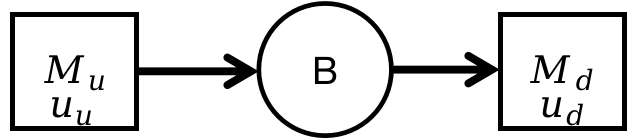
\includegraphics[width=0.3\textwidth]{figures/two_machine_line.png} 
    \caption{Material accumulating in buffer}
    \label{fig:two_machine_line}
\end{figure}
Time to fulfillment $RB \lbrace b, tf \rbrace$ and time to depletion $RB \lbrace b, td \rbrace$ can be measure by equation \ref{buffer_full} and \ref{buffer_empty}.
\begin{equation}\label{buffer_full}
    RB \lbrace b, tf \rbrace = \frac{N \lbrace b \rbrace - x \lbrace b \rbrace}{\mu_u - \mu_d}
\end{equation}
\begin{equation}\label{buffer_empty}
    RB \lbrace b, td \rbrace = \frac{L \lbrace b \rbrace - x \lbrace b \rbrace}{\mu_u - \mu_d}
\end{equation}
For a long transfer lines more than once buffer can be filled or emptied this results in accelerating the blocking and starvation of modules, this phenomenon can be addressed by propagation. 

\subsection{Propagation}
In figure \ref{tab:propagation} we can see a long line, the color of the module is related the processing speed of machine or module. The dark green represents a higher processing rate and lighter color indicates a lower processing rate respectively. In case of $blocking$ buffer $B3$ gets filled first (represented in dark blue color) and this forces module $M_{3}$ to operate at lower processing than its ideal processing rate. Since the flow should accept the continuity of material the update processing rate of module three $\mu^{update}_{3}$ should equal to $\mu^{ideal}_{4}$. If we assume all the modules will not fail in near future this will force $B2$ to fill, hence blocking $M_{2}$. Applying the continuity condition the processing rate for second modules should be updated as $\mu^{update}_{2} = \mu^{updated}_{3}$. This phenomenon can be termed as propagation. Similarly, the propagation of starvation is also showed in figure \ref{tab:propagation} on right side. The red color represents the buffer getting empty. \par
\begin{table}[htbp]
    \centering
    \begin{tabular}{|p{6cm}|p{6cm}|}
        \hline
        Blocking & 
        Starvation\\
        \hline  
        \parbox[c]{2cm}{\centering 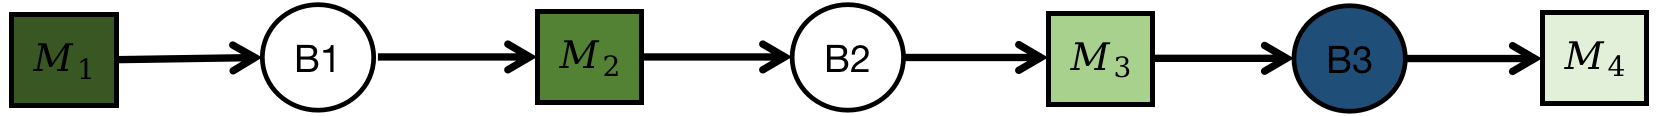
\includegraphics[width = 
        6cm]{figures/b1.png}} &
        \parbox[c]{2cm}{\centering 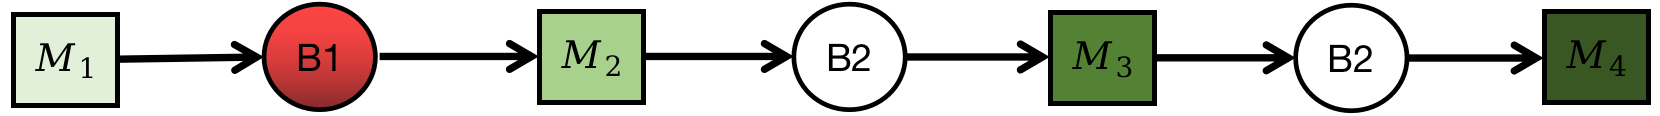
\includegraphics[width = 6cm]{figures/s1.png}} \\
        \parbox[c]{2cm}{\centering 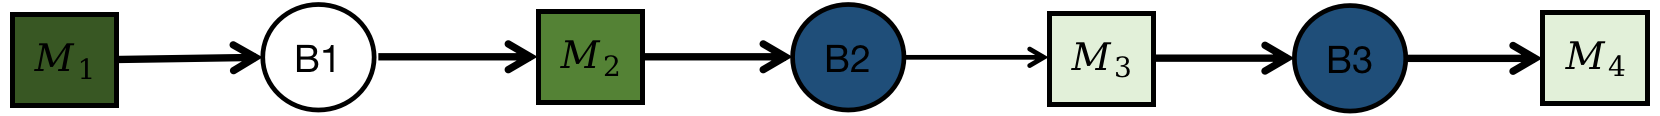
\includegraphics[width = 
        6cm]{figures/b2.png}} &
        \parbox[c]{2cm}{\centering 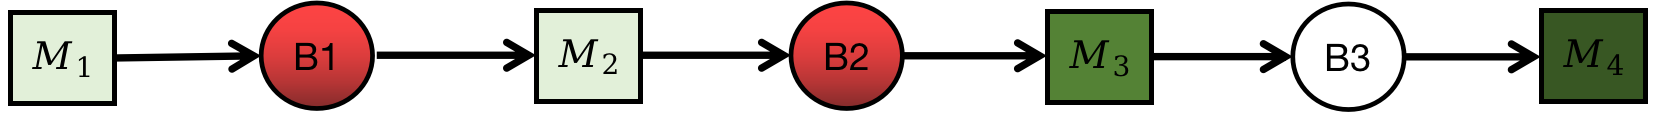
\includegraphics[width = 6cm]{figures/s2.png}} \\
        \parbox[c]{2cm}{\centering 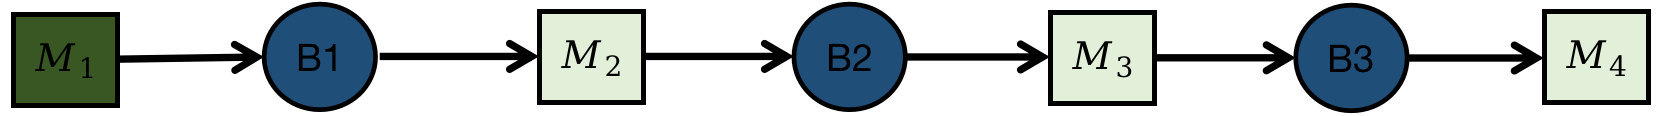
\includegraphics[width = 
        6cm]{figures/b3.png}} &
        \parbox[c]{2cm}{\centering 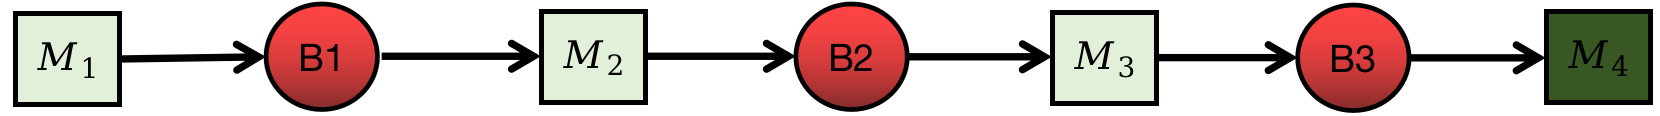
\includegraphics[width = 6cm]{figures/s3.png}} \\
        \parbox[c]{2cm}{\centering 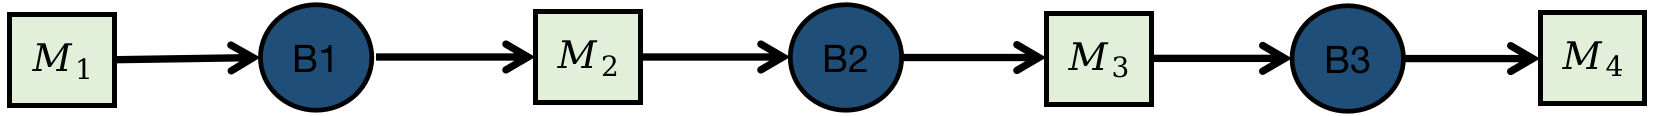
\includegraphics[width = 
        6cm]{figures/b4.png}} &
        \parbox[c]{2cm}{\centering 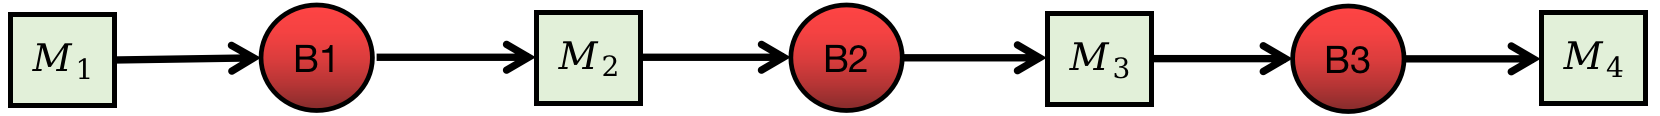
\includegraphics[width = 6cm]{figures/s4.png}} \\
        \hline  

    \end{tabular}
    \caption{Propagation of blocking and starvation in a transfer line.}
    \label{tab:propagation}
\end{table}
In case of blocking, after certain time all the buffers will be filled forcing all the upstream modules to operate with the processing rates of the downstream modules. For Starvation the modules down the stream are forced affected due to the lower processing rates of upstream machines. In our algorithm, we address this phenomenon by changing the processing rates of the modules based on the buffer level on upstream and downstream to machine. \par 
Now we have all the pieces to stitch, the algorithm for building a continuous simulation is presented in algorithm \ref{alogo_contiunous_simulation}. The simulation starts at current time $t_{k} = 0$ the next event in the system can be obtained as $\Delta t = min(RM \lbrace m \rbrace, RB \lbrace b \rbrace)$. The next step is to update the state space of the system by this $\Delta t$. The update step involves computing the buffer levels, updating the failure matrix and propagation in case of blocking or starvation. 

\begin{algorithm}
    \KwData{Production graph with parameters for modules and buffers. \par $run$ $time$  = $t_{simulation}$}
    \KwResult{Average buffer levels and throughput}
    initialization\;
    $t_{k} = 0 $ \;
    \While{$t_{k} < t_{simulation}$}{
        \textbf{compute events}\par
        $RM\lbrace m \rbrace$ = compute module events \;
        $RB\lbrace m \rbrace$ = compute buffer events \;
        \hspace{10pt}$t_{k+1} = t_{k} + \min({RM \lbrace m \rbrace, RB \lbrace m \rbrace})$ \;
        \textbf{update state}\par
        compute buffer levels \par
        \hspace{10pt}$x^b(t_{k+1}) = x^b(t) + (\mu_{u} - \mu_{d}) * \Delta t$ \par
        update module state \par 
        \hspace{10pt} $\mu_{m}$ - Processing rates\par
        \hspace{10pt} $FM_{m}$ - Failure matrix\par
        Propagation to update processing rates.
    }
    \caption{Algorithm for continuous simulation}\label{alogo_contiunous_simulation}
\end{algorithm}